% !TEX program = xelatex
\documentclass[hyperref,a4paper,UTF8]{ctexart}

\usepackage[left=2.50cm, right=2.50cm, top=2.50cm, bottom=2.50cm]{geometry}

\usepackage[unicode=true,colorlinks,urlcolor=blue,linkcolor=blue,bookmarksnumbered=true]{hyperref}
\usepackage{latexsym,amssymb,amsmath,amsbsy,amsopn,amstext,amsthm,amsxtra,color,bm,calc,ifpdf}
\usepackage{graphicx}
\usepackage{enumerate}
\usepackage{fancyhdr}
\usepackage{listings}
\usepackage{multirow}
\usepackage{makeidx}
\usepackage{xcolor}
\usepackage{fontspec}
\usepackage{subfigure}
\usepackage{hyperref}
\usepackage{pythonhighlight}
\usepackage{pdfpages}
\usepackage{tabularx}
\usepackage{booktabs}
\usepackage{amsthm}
\usepackage{amssymb}
\usepackage{mathrsfs}
\usepackage{tikz}


\newtheorem{theorem}{定理}[section]
\newtheorem{lemma}{Lemma}[section]
\newtheorem{corollary}{Corollary}[section]
\newtheorem{definition}{定义}[section]
\newtheorem{proposition}{{命题}}
\newtheorem{property}{{性质}}


% \linespread{0.8}\selectfont

% \lstset{numbers=left, 
%         numberstyle= \tiny, 
%         keywordstyle= \color{ blue!70},%设置关键字颜色
%         commentstyle= \color{red!50!green!50!blue!50}, %设置注释颜色
%         frame=shadowbox, % 阴影效果
%         rulesepcolor= \color{ red!20!green!20!blue!20} ,
%         escapeinside=``, % 英文分号中可写入中文
%         xleftmargin=2em, %距离左边界2em
%         aboveskip=1em,
%         framexleftmargin=2em,
%         basicstyle=\ttfamily,
%         columns=fullflexible,%可以自动换行
%         linewidth=1\linewidth, %设置代码块与行同宽
%         breaklines=true,%在单词边界处换行。
%         showstringspaces=false, %去掉空格时产生的下划的空格标志, 设置为true则出现
%         breakatwhitespace=ture,%可以在空格处换行
%         escapechar=`%设置转义字符为反引号
%         }

%---------- matlab and python code style ----------
% Matlab highlight color settings
%\definecolor{mBasic}{RGB}{248,248,242}       % default
\definecolor{mKeyword}{RGB}{0,0,255}          % bule
\definecolor{mString}{RGB}{160,32,240}        % purple
\definecolor{mComment}{RGB}{34,139,34}        % green
\definecolor{mBackground}{RGB}{245,245,245}   % lightgrey
\definecolor{mNumber}{RGB}{128,128,128}       % gray

% Python highlight color settings
%\definecolor{pBasic}{RGB}{248, 248, 242}     % default
\definecolor{pKeyword}{RGB}{228,0,128}        % magenta
\definecolor{pString}{RGB}{148,0,209}         % purple
\definecolor{pComment}{RGB}{117,113,94}       % gray
\definecolor{pIdentifier}{RGB}{166, 226, 46}  %
\definecolor{pBackground}{RGB}{245,245,245}   % lightgrey
\definecolor{pNumber}{RGB}{128,128,128}       % gray

\lstdefinestyle{matlab}{
  language=matlab,               % choose the language of the code
  xleftmargin=25pt,
  xrightmargin=15pt,
  frame=tlbr,framesep=4pt,framerule=0pt, % sets the frame style
  %frame=shadowbox,rulesepcolor=\color{red!20!green!20!blue!20},
  basicstyle=\small\ttfamily,
  keywordstyle={\color{mKeyword}},     % sets color for keywords
  stringstyle={\color{mString}},       % sets color for strings
  commentstyle={\color{mComment}},     % sets color for comments
  backgroundcolor=\color{mBackground}, % choose the background color
  %title=#1,                            % \lstname show the filename of files
  keywords={break,case,catch,classdef,continue,else,elseif,end,for,
  function,global,if,otherwise,parfor,persistent,return,spmd,switch,try,while},
  showspaces=false,                    % show spaces adding particular underscores
  showstringspaces=false,              % underline spaces within strings
  showtabs=false,                      % show tabs within strings adding particular underscores
  tabsize=4,                           % sets default tabsize to 2 spaces
  captionpos=t,                        % sets the caption-position to bottom
  breaklines=true,                     % sets automatic line breaking
  numberstyle=\tiny\color{mNumber},
  numbers=left,                        % where to put the line-numbers
  stepnumber=1,                        % the step between two line-numbers.
  %numbersep=5pt,                      % how far the line-numbers are from the code
}

\lstdefinestyle{python}{
  language=python,               % choose the language of the code
  xleftmargin=25pt,
  xrightmargin=15pt,
  frame=tlbr,framesep=4pt,framerule=0pt, % sets the frame style
  %frame=shadowbox,rulesepcolor=\color{red!20!green!20!blue!20},
  %basicstyle=\small\ttfamily,          % sets font style for the code
  basicstyle=\footnotesize\fontspec{Consolas},
  keywordstyle=\color{pKeyword},       % sets color for keywords
  stringstyle=\color{pString},         % sets color for strings
  commentstyle=\color{pComment},       % sets color for comments
  backgroundcolor=\color{pBackground}, % choose the background color
  %title=#1,                            % \lstnames how the filename of files
  emph={format_string,eff_ana_bf,permute,eff_ana_btr},
  emphstyle=\color{pIdentifier}
  showspaces=false,                    % show spaces adding particular underscores
  showstringspaces=false,              % underline spaces within strings
  showtabs=false,                      % show tabs within strings adding particular underscores
  tabsize=4,                           % sets default tabsize to 2 spaces
  captionpos=t,                        % sets the caption-position to bottom
  breaklines=true,                     % sets automatic line breaking
  numberstyle=\tiny\color{pNumber},
  numbers=left,                        % where to put the line-numbers
  stepnumber=1,                        % the step between two line-numbers.
  %numbersep=5pt,                      % how far the line-numbers are from the code
}


%链接颜色设置
\hypersetup{colorlinks=true,linkcolor=black}

\pagestyle{fancy}
\fancyhead[L]{}
\fancyhead[C]{\fangsong Hausdorff测度简介}
\fancyhead[R]{}

\renewcommand{\abstractname}{\textbf{\large {摘\quad 要}}} % 更改摘要二字的样式


\title{\textbf{{Hausdorff测度简介}}}
\author{
\kaishu\normalsize
姓名\ \underline{梁津滏} \qquad
学号\ \underline{238612090034} \qquad
% 院系\ \underline{数学学院}
任课老师\ \underline{郑云瑞}
}
\date{\today} % 留空,不显示日期


\begin{document}

\begin{figure}
    \centering
    
\includegraphics[width=0.65\textwidth]{figure/SDU.jpg}
\end{figure}

\maketitle

\begin{abstract}

本文主要介绍了Hausdorff测度的基本内容 . 

首先,我们从Hausdorff外测度的定义出发,叙述了外测度的定义形式. 然后我们介绍了Hausdorff测度的基本性质. 在Hausdorff测度的基础上,定义了Hausdorff可测集,并给出了Hausdorff可测集的基本性质.最后,我们给出Hausdorff维数的定义, 以Cantor集为例,证明了Cantor集的Hausdorff维数为$\frac{\mathrm{ln}2}{\mathrm{ln}3}$.最后,我们给出Minkowski维数的定义,证明Minkowski维数不小于Hausdorff维数.

\end{abstract}

\thispagestyle{empty} % 当前页不显示页码
\newpage

\tableofcontents

\thispagestyle{empty} % 当前页不显示页码
\newpage



%--------------------------------------------分割线----------------------------------------------------------------------------------------

\section{引言}

按照$R^n$中的Lebesgue测度,是无法区别$R^n$内的两个零测集的.
但这些几何在分形几何及动力系统以及其他一些学科中是十分重要的.
于是出现了所谓分数维数(Hausdorff维数)概念. 

\section{Hausdorff外测度}

\subsection{Hausdorff外测度的定义}

\begin{definition}
  对$\mathbb{R}^d$的任何子集E,
  记 $\mathcal{H}^{\alpha}_{\delta}(E) = inf \left\{\sum\left(\mathrm{\mathrm{diam}} F_k\right)^\alpha: E \subset \bigcup\limits_{k=1}^{\infty} F_k, \mathrm{diam} F_k \leqslant \delta \text {, 对所有 } k\right\} \text {. }$
  称$\mathcal{H}^{\alpha}(E)=\lim\limits_{\delta  \to 0}\mathcal{H}^{\alpha}_{\delta}(E)$为Hausdorff外测度.
  其中,$\mathrm{diamS} = \mathrm{sup}{|x-y|:x,y \in S}$. 
\end{definition}

\begin{proposition}
  Hausdorff外测度是一个测度.
\end{proposition}

要证明Hausdorff外测度是一个测度,只需证明$\mathcal{H}^{\alpha}(E)$是非负的,且有可数可加性. 
\begin{proof}
   $\mathcal{H}^{\alpha}(E) \geqslant 0$, 这根据定义是显然的.

  根据后文中的次可加性,Hausdorff外测度是一个测度. 这里错了,要可数可加性,不是次可加性.
\end{proof}


\subsection{性质}
  \begin{property}
    若$E_1 \subset E_2 $,则$\mathcal{H}^{\alpha}(E_1) \leq \mathcal{H}^{\alpha}(E_2)$.
  \end{property}
  \begin{proof}
    因为$E_2$的任何覆盖也是$E_1$的覆盖,所以这个性质显然成立.
  \end{proof}

    %--------------------------------------------------------------
  \begin{property}[次可加性]
    对$\mathbb{R}^d$中的任何可数集簇${E_j}$,有$\mathcal{H}^{\alpha}\left(\bigcup_{j=1}^{\infty} E_j\right) \leqslant \sum_{j=1}^{\infty} \mathcal{H}^{\alpha}\left(E_j\right)$. 
  \end{property}
  \begin{proof}
    先固定 $\delta$, 对每个 $j$ 选择 $E_j$ 的一个用直径小于 $\delta$ 的集合的覆盖 
    $\left\{F_{j, k}\right\}_{k=1}^{\infty}$, 使得 
    
    $\sum\limits_k\left(\mathrm{diam} F_{j, k}\right)^\alpha \leqslant \mathcal{H}_\delta^\alpha\left(E_j\right)+\varepsilon / 2^j$ .
    由于 $\bigcup\limits_{j, k} F_{j, k}$ 是 $E$ 的一个直径小于 $\delta$ 的集合的并的覆盖, 故有
    $$
      \begin{aligned}
        \sum_{j}\sum\limits_k\left(\mathrm{diam} F_{j, k}\right)^\alpha & \leqslant \sum_{j} \left \{\mathcal{H}_\delta^\alpha\left(E_j\right)+\varepsilon / 2^j \right \}\\
        \mathcal{H}_\delta^\alpha(E) & \leqslant \sum_{j=1}^{\infty} \mathcal{H}_\delta^\alpha \left(E_j\right)+\varepsilon \\
        \mathcal{H}^\alpha(E) & \leqslant \sum_{j=1}^{\infty} \mathcal{H}^\alpha\left(E_j\right)+\varepsilon 
      \end{aligned}
    $$
    %--------------------------------------------------------------
    由于 $\varepsilon$ 是任意的, 不等式 $\mathcal{H}^\alpha(E)\leqslant \sum_{j=1}^{\infty} \mathcal{H}^\alpha\left(E_j\right)$ 成立.
  \end{proof}

  \begin{property}
    $\mathcal{H}^\alpha(A) = 0$ $\Leftrightarrow$
      $ \forall \varepsilon > 0, \exists E_{1}, E_{2}, \cdots \in  \mathbb{R}^{n}\text{, s.t.} A \subseteq \bigcup\limits_{i} E_{i}$ 且 $\sum_{i}\left(\mathrm{diam}\left(E_{i}\right)\right)^{\alpha}<\varepsilon$ . 
  \end{property}
  \begin{proof}
      $ \Rightarrow) \mathcal{H}^\alpha_\delta(E) = inf \left\{\sum\limits_{i}\left(\mathrm{diam} F_i\right)^\alpha: E \subset \bigcup\limits_{i=1}^{\infty} F_i, \mathrm{diam} F_i \leqslant \delta, \forall i\right\}$. 

      由$ \mathcal{H}^\alpha(A) = \lim\limits_{\delta \to 0} \mathcal{H}_\delta^\alpha(A) = 0$知, $\forall i,A \subset \bigcup\limits_{i=1}^{\infty} E_i, \mathrm{diam} E_i \leqslant \delta, \sum\limits_{i}\left(\mathrm{diam}\left(E_{i}\right)\right)^{s}<\varepsilon$
      
      就取这些$E_i$,使得$\sum\limits_{i}\left(\mathrm{diam}\left(E_{i}\right)\right)^{s}<\varepsilon$成立.

      反之,$ \forall \varepsilon > 0, \exists E_{1}, E_{2}, \cdots \in  \mathbb{R}^{n}\text{, s.t.} A \subseteq \bigcup\limits_{i} E_{i}$ 且 $\sum_{i}\left(\mathrm{diam}\left(E_{i}\right)\right)^{\alpha}<\varepsilon$. 
      那么 ,取这些子集$E_{1}, E_{2}, \cdots$,就可以得到$\mathcal{H}^\alpha_M(A) = inf \left\{\sum_{i}\left(\mathrm{diam} E_i\right)^\alpha: E \subset \bigcup_{i=1}^{\infty} E_i, \mathrm{diam} E_i \leqslant M,\forall i,\text{M 足够大}\right\} < \varepsilon$.由于 $\varepsilon$ 是任意的, 所以 $0 \leqslant \mathcal{H}^\alpha(A) \leqslant \mathcal{H}^\alpha_M(A) \leqslant 0 $, 故 $\mathcal{H}^\alpha(A) = 0$.

  \end{proof}
      % \item \textbf{性质4}:
    % 对于任何 $c > 0$ 和集合 $E \subseteq X$,
    % \[
    % \mathcal{H}^s(cE) = c^s \mathcal{H}^s(E)
    % \]
    % 这里,$cE = \{cx : x \in E\}$。

    % \item \textbf{零维和正维的关系}:
    % 对于任意集合 $E \subseteq X$,存在一个唯一的值 $s$ 使得
    % \[
    % \mathcal{H}^t(E) = \begin{cases} 
    % \infty, & \text{如果 } t < s, \\
    % 0, & \text{如果 } t > s 
    % \end{cases}
    % \]
    % 这个唯一的值 $s$ 被称为集合 $E$ 的 Hausdorff 维度。

    % \item \textbf{与 Lebesgue 测度的关系}:
    % 在欧几里得空间 $\mathbb{R}^n$ 中,对于整数 $s = n$,$n$ 维 Hausdorff 测度 $\mathcal{H}^n$ 与 Lebesgue 测度等价(至一个常数因子)。

    % \item \textbf{正则性}:
    % 对于测度为有限的集合,$\mathcal{H}^s$ 是外正则和内正则的。





\section{Hausdorff可测集}

Lebesgue可测集借助Lebesgue外测度来定义. 
抽象测度具备更广泛的适用范围,下面将列出抽象测度的定义.
仿照Lebesgue可测集和抽象测度的可测集,我们定义Hausdorff可测集.

\begin{definition}[Lebesgue 外测度]

  设 $E$ 是 $\mathbb{R}^n$ 的点集,$\{I_n\}_{n=1}^{\infty}$ 是 $\mathbb{R}^n$ 中的一列开长方体,且 $\bigcup\limits_{n=1}^{\infty} I_n \supseteq E$。则 $\sum\limits_{n=1}^{\infty} |I_n|$ 确定一个非负的数 $u$(或 $+\infty$)。记
  \[ 
  m^*(E) = \inf \left\{ u \mid u = \sum_{n=1}^{\infty} |I_n| , \bigcup_{n=1}^{\infty} I_n \supseteq E, I_n \text{ 是开长方体} \right\} 
  \]
  称 $m^*(E)$ 为 $E$ 的 Lebesgue 外测度.
\end{definition}

\begin{definition}[Lebesgue 可测集]

  假设 \( E \subset \mathbb{R}^n \),如果对任何集合 \( T \subset \mathbb{R}^n \) 都有
  \[ 
  m^*(T) = m^*(T \cap E) + m^*(T \cap E^c), 
  \]
  则称 \( E \) 为 Lebesgue 可测集,此时称 \( m^*(E) \) 为 \( E \) 的 Lebesgue 测度。
\end{definition}

% 抽象测度定义
%% 环的定义
\begin{definition}[$\sigma$ - 环]

  设$\mathscr{R}$ 是非空集合S的一簇非空子集,如果存在

  (1) 当 $A,B\in \mathscr{R}$ 时, 有 $A \cup B \in \mathscr{R}$;

  (2) 当 $A,B\in \mathscr{R}$ 时, 有 $A - B \in \mathscr{R}$,

  则称$\mathscr{R}$是S的子集构成的一个环.如果还有

  (3)对任意$A_n \in \mathscr{R}$,

  $n = 1,2,3,\cdots$,有

  \[
  \bigcup_{n=1}^{\infty} A_n \in \mathscr{R}
  \]
  
  则称$\mathscr{R}$是S的子集构成的$\sigma$ - 环.

\end{definition}
%抽象测度可测定义

\begin{definition}[可加与可数可加]

  设$\mathscr{R} 是环,\mu : \mathscr{R} \rightarrow \mathbb{R}$ 是映射,
  如果对任意$A,B \in \mathscr{R}$,
  只要$A \cap B = \varnothing $,则有$\mu(A\cap B) = \mu(A) + \mu(B)$,
  则称$\mu$ 是可加的. 

  如果当$A_n \in \mathscr{R}, n = 1,2,3,\cdots$ 互不相交
  且$ \bigcap\limits_{n=1}^{\infty} A_n \in \mathscr{R}$ 时,
  有 
  

  \[
    \mu\left(\bigcup_{n=1}^{\infty} A_{n}\right) = \sum_{n=1}^{\infty} \mu\left(A_{n}\right)
  \]
  则称$\mu$ 是可数可加的.


\end{definition}

\begin{definition}[测度]

  假如对于任意集合$A \in \mathscr{R}$, $\mu(A) \geq 0$, 则称 $\mu $是非负的. 
  $\mathscr{R}$上非负的可数可加的使$\mu(\varnothing) = 0$的集合函数称为$\mathscr{R}$上的一个测度. 

\end{definition}

\begin{definition}[可测]

  设$A\in\mathscr{R}$,若对任意$T \in \mathscr{R}$,等式
  \[
    \mu^*(T) = \mu^*(T \cap A) + \mu^*(T \cap A^C) 
  \]

  恒成立,则称$A$为$\mu^*-\text{可测集}$.
  要寄!!!!!!

\end{definition}

\subsection{定义}

仿照 Lebesgue 可测集的定义, 定义 Hausdorff 可测集如下:

\begin{definition}[Hausdorff 可测集]
  $ \mathcal{H}^s(A) = \lim\limits_{\delta \to 0} \mathcal{H}_\alpha^\delta(A)$.
  假设 \( E \subset \mathbb{R}^n \),如果对任何集合 \( T \subset \mathbb{R}^n \) 都有
  \[ 
    \mathcal{H}^s(T) = \mathcal{H}^s(T \cap E) + \mathcal{H}^(T \cap E^c), 
  \]
  则称 \( E \) 为 Hausdorff 可测集,此时称 \( \mathcal{H}^s(E) \) 为 \( E \) 的 Hausdorff 测度.\textrm{\textcolor{red}{(2)}}
\end{definition}

\subsection{性质}

\begin{enumerate}

  \item \textbf{性质:单调性}:若$E_1 \subset E_2$,则$\mathcal{H}^s(E_1) \leqslant \mathcal{H}^s(E_2)$.

  \begin{proof}
    因为$E_2$的任何覆盖也是$E_1$的覆盖,所以这个性质显然成立.
  \end{proof}

  \item \textbf{性质:次可加性}:对$\mathbb{R}^n$中的任意可数集簇${E_j}$,有$\mathcal{H}^s\left(\bigcup\limits_{j=1}^{\infty} E_j\right) \leqslant \sum_{j=1}^{\infty} \mathcal{H}^s\left(E_j\right)$.
  \begin{proof}
    先固定$\delta$,对于每个$j$选择$E_j$的一个直径小于$\delta$的集合的覆盖$\left \{  F_{j,k} \right \}^{\infty}_{k=1}$,使得
    $$\sum_k(\mathrm{diam}F_{j,k})^{\alpha}\leqslant \mathcal{H}_\delta^\alpha(E_j)+\frac{\varepsilon}{2^j} $$
    由于$\bigcup\limits_{j,k} F_{j,k}$是E的一个直径小于$\delta$的集合的覆盖,故有
    \begin{align*}
      \mathcal{H}_\delta^\alpha(E) & \leqslant \sum_{j=1}^{\infty} \mathcal{H}_\delta^\alpha(E_j)+\varepsilon \\
      & \leqslant \sum_{j=1}^{\infty} \mathcal{H}^\alpha(E_j)+\varepsilon. 
    \end{align*}
    由于$\varepsilon$是任意的,不等式$\mathcal{H}_\delta^\alpha(E) \leqslant \sum \mathcal{H}_\delta^\alpha(E_j)$成立,令$\delta$趋于0就证明了$\mathcal{H}_\delta^\alpha$的可数次可加性.
  \end{proof}
  
  \item \textbf{性质}:设$A,B \subseteq \mathbb{R}^n$ ,且 $d(A, B)>0$.
   则$\mathcal{H}^{s}(A \cup B)=\mathcal{H}^{s}(A)+\mathcal{H}^{s}(B)$.

  \begin{proof}
    $\mathcal{H}^{s}(A \cup B)\leqslant \mathcal{H}^{s}(A)+\mathcal{H}^{s}(B)$由上一条性质直接得到.

    下面证明$\mathcal{H}^{s}(A \cup B)\geqslant \mathcal{H}^{s}(A)+\mathcal{H}^{s}(B)$. 

    固定 $\varepsilon > 0 $满足 $\varepsilon \le d(F_1, F_2)$. 令 $\delta < \varepsilon$ ,用$F_1, F_2, F_3, \cdots$ 覆盖$E_1\cup E_2$. 
    令

    \[
      F_j' = E_1 \cap F_j, F_j{''} = E_2 \cap F_j. 
    \]

    ${F_j'}$和${F_j{''}}$是$E_1$和$E_2$的互不相交的覆盖. 
    因此

    \[
      \sum_j (\mathrm{diam} F_j')^{\alpha}+\sum_i (\mathrm{diam} F_i{''})^{\alpha} \leqslant \sum_k (\mathrm{diam} F_k)^{\alpha}
    \]

    \[
      \mathrm{inf} \sum_j (\mathrm{diam} F_j')^{\alpha}+\mathrm{inf}\sum_i (\mathrm{diam} F_i{''})^{\alpha} \leqslant \mathrm{inf}\sum_k (\mathrm{diam} F_k)^{\alpha}
    \]

    \[
        \mathcal{H}^{s}(A)+\mathcal{H}^{s}(B) \leqslant \mathcal{H}^{s}(A \cup B)
    \]



  \end{proof}
\end{enumerate}

\subsection{定理}

\begin{theorem}
  
  所有Borel集都是Hausdorff可测集.

\end{theorem}

\begin{proof}
  1. Borel集的构造

  由$\mathrm{R}^n$中的开集经过可数次的交、并、差运算后得到的$\sigma -$ 域 记作$ \mathcal{B}(\mathbb{R}^n)$,
  称为$\mathbb{R}^n$中的Borel集类.$\mathcal{B}$中的元称为Borel集. 
  由于根据Hausdorff可测集的性质,开集有限次交、并、差运算后得到的集合仍是可测集. 
  因此,我们只需要证明,任何开集Hausdorff可测.

  2.任何开集Hausdorff可测

  设$E \subset \mathbb{R}^n$ 为开集. 不妨设$G = \varnothing $.
  则G可以写成无数个互不相交的区间之并
  $\bigcup\limits_{i=1}^{\infty} E_i$. 我们可以保证这些区间都是可测的. 

  再由可测集的可数次交并补运算仍然是可测集,得到任意的开集Hausdorff可测.

\end{proof}

\section{Hausdorff 维数}

\subsection{定义}
\begin{definition}
  假设 \( E \subset \mathbb{R}^n \),定义E的Hausdorff维数为

  \[
    \mathrm{dim} E = \inf\{s \in \mathbb{R}^1: \mathcal{H}^{s}(E) = 0 \}.
  \]

\end{definition}

\begin{definition}[Minkowski 维数]

\end{definition}


\subsection{性质}
%命题
\begin{proposition}

  Cantor集的Hausdorff维数为$\dfrac{\mathrm{ln}2}{\mathrm{ln}3}$. 
\end{proposition}

\begin{proof}
Cantor集的构造为将[0,1]均分为3段,去掉中间的开区间. 然后将剩下的两个区间分别做三等分,分别去掉中间的开区间. 这样继续下去,最终留下的点集记作C. 

\begin{figure}[htbp]
  \centering
  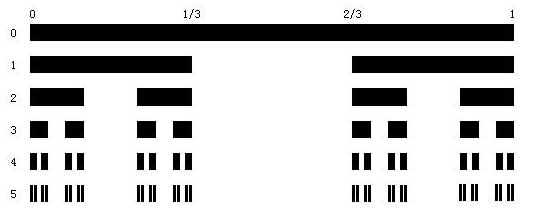
\includegraphics[width=0.5\textwidth]{image/cantor.jpg}
  \caption{Cantor集}
\end{figure}

记第一次分割$[0,1]$得到的闭集为$C_1$,第二次得到的集合为$C_2$,一直划分$n$次,得到集合$C_n$. 

\begin{table}[htbp]
  \centering
  \caption{康托集的性质}
  \begin{tabular}{ccc}
  \toprule
  集合 & Lebesgue测度 & 不交的闭集个数 \\
  \midrule
  $C_1$ & $\frac{2}{3}$ & $2^1$ \\
  $C_2$ & $\left(\frac{2}{3}\right)^2$ & $2^2$ \\
  $\vdots$ & $\vdots$ & $\vdots$ \\
  $C_n$ & $\left(\frac{2}{3}\right)^n$ & $2^n$ \\
  \bottomrule
  \end{tabular}
\end{table}

记 $C = \bigcup\limits_{i=1}^{\infty} C_i$, C是有界闭集. 

C的Lebesgue测度为0. 

\[
\mu(C) = \frac{2}{3}+\left(\frac{2}{3}\right)^2+\cdots+\left(\frac{2}{3}\right)^n=\frac{2}{3}\left(1-\frac{1}{3}\right)^n
\]

\[
\begin{aligned}
  \mu(C) &= \mu\left(\bigcap_{i=1}^{\infty} C_i\right) \\
  &= \lim\limits_{n \rightarrow \infty} \mu(C_n) \\
  &=  \lim\limits_{n \rightarrow \infty}2^{n}\frac{1}{3^{n\alpha}}\\
  &= 0
\end{aligned}
\]

下证C的Hausdorff维数为$\dfrac{\mathrm{ln}2}{\mathrm{ln}3}$.

\[
\begin{aligned}
  \mathcal{H}^\alpha(C) &= \lim\limits_{\delta \rightarrow 0}\mathrm{inf}\left \{ \sum_{k}(\mathrm{diam}F_k)^{\alpha} \vert C \subset \bigcup\limits_{k} F_k , \forall F_k\in \mathbb{R}^n, F_k \le \delta \right \} \\
  &= \lim\limits_{n \rightarrow \infty}\left \{\frac{2}{3^\alpha} \right \}^{n} \\
  &\leqslant \mathcal{H}^\alpha(C)\\
  &= \left \{\frac{2}{3^\alpha} \right \}^{k}
\end{aligned}  
\]

令 $3^\alpha = 2$, 则
$\alpha = \dfrac{\mathrm{ln}2}{\mathrm{ln}3}$, 此时 $\mathcal{H}^\alpha(C) \leqslant 1 $ . 

下面证明 $\mathcal{H}^\alpha(C)$有下界.

构造Cantor-Lebesgue函数. 

\begin{figure}[htbp]
  \centering
  \begin{minipage}{0.3\textwidth}
      \centering
      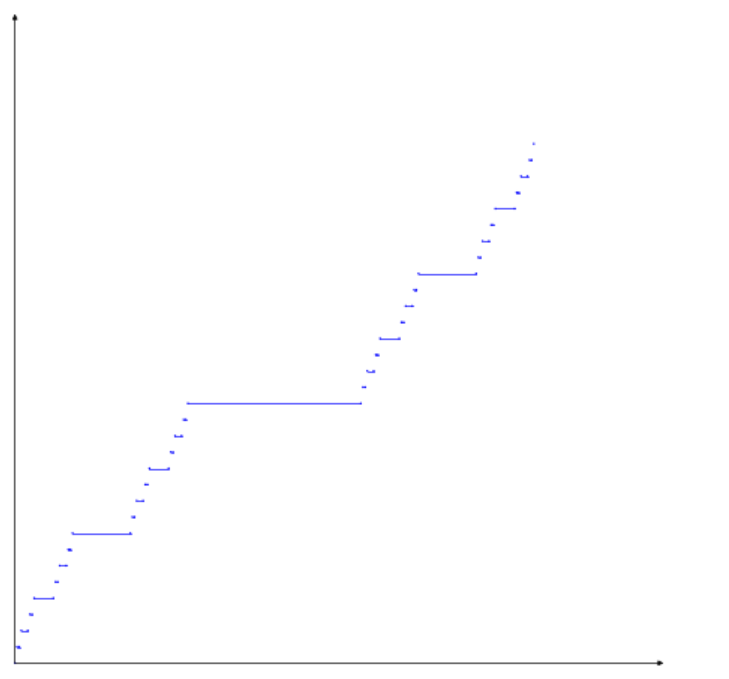
\includegraphics[width=\textwidth]{image/cantor_lebesgue.png}
  \end{minipage}
  \begin{minipage}{0.3\textwidth}
      \centering
      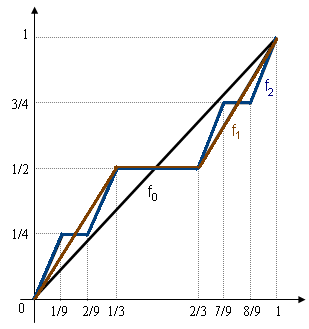
\includegraphics[width=\textwidth]{image/Cantor_function_sequence.png}
  \end{minipage}
\end{figure}


下面我们构造一个函数序列 $\{f_n(x)\}$,这个序列将收敛于Cantor-Lebesgue函数函数.
首先定义
\[
f_0(x) = x
\]
接下来,对于每个正整数 $n$,函数 $f_{n+1}(x)$ 都由函数 $f_n(x)$ 定义:
\[
f_{n+1}(x) = 
\begin{cases}
    \frac{1}{2} \times f_n(3x) & \text{if } 0 \leq x < \frac{1}{3} \\
    \frac{1}{2} & \text{if } \frac{1}{3} \leq x < \frac{2}{3} \\
    \frac{1}{2} + \frac{1}{2} \times f_n(3x-2) & \text{if } \frac{2}{3} \leq x \leq 1
\end{cases}
\]

\[
 \vert f_2(x) - f_1(x) \vert \le \frac{1}{2^2}
\]

\[
 \vert f_3(x) - f_2(x) \vert \le \frac{1}{2^3}
\]

\[
  \cdots
\]

\[
 \vert f_n(x) - f_{n-1}(x) \vert \le \frac{1}{2^n}
\]

注意到,$\vert f_{n+p}(x) - f_{n}(x) \vert \leqslant  \vert f_{n+p}(x) - f_{n+p-1}(x) \vert + \dots +\vert f_{n+1}(x) - f_{n}(x) \vert$. 
故$\forall \varepsilon > 0,\exists N,p > 0,\forall n > N,\vert f_{n+p}(x) - f_{n}(x) \vert \leqslant  \vert f_{n+p}(x) - f_{n+p-1}(x) \vert + \dots +\vert f_{n+1}(x) - f_{n}(x) \vert < \frac{1}{2^n} < \varepsilon$. 

因此在$x \in [0,1]$上,$f_n \rightrightarrows f$. 

下面先证明Cantor-Lebesgue函数Hölder连续. 

定义
$\forall x_1, x_2 \in [0,1] , \text{若}\exists \gamma \in \mathbb{R}^+,\vert f(x_1) - f(x_2) \vert \le M \vert x_1-x_2 \vert^\gamma$,则f是$\gamma$-Hölder连续.  
\begin{align*}
  \vert f(x_1) - f(x_2) \vert &\le \vert f(x_1) - f_n(x_1) \vert+\vert f_n(x_1) - f_n(x_2) \vert+\vert f_n(x_1) - f(x_2) \vert\\
  &\le \frac{1}{2^n}+\frac{3}{2}^n \vert x_1-x_2 \vert + \frac{1}{2^n}
\end{align*}

对于给定的$\vert x_1-x_2 \vert$,可以选取n, $\text{s.t.} 1 \leqslant 3^n\vert x_1-x_2 \vert \leqslant 3,$
\begin{align*}
\vert f(x_1) - f(x_2) \vert &\leqslant C \frac{1}{2^n} \\
&\leqslant C \frac{3^{n\gamma}}{2^n}\frac{1}{3^{n\gamma}}\\
&\leqslant C \frac{3^{n\gamma}}{2^n} \vert x_1-x_2 \vert^\gamma \quad (\text{令}\gamma = \frac{\mathrm{ln}2}{\mathrm{ln}3}) \\
& = C\vert x_1-x_2 \vert^{\frac{\mathrm{ln}2}{\mathrm{ln}3}}
\end{align*}

所以f是$\dfrac{\mathrm{ln}2}{\mathrm{ln}3}$-Hölder连续. 


考虑 $\phi (x)$ 在E上有定义. $\vert \phi (x) - \phi (y) \vert \leqslant M \vert x-y \vert^\gamma,\forall x,y \in E.$ 

$\forall F,F \subset \bigcup\limits_{i=1}^{\infty} E_i, \mathrm{diam}E_i<\delta $ ,
$\Phi(F) \subset \bigcup\limits_{i=1}^{\infty}\phi(F \cap E_i)$. 

可以由$\phi$ 的$\gamma$-Hölder连续性推出F和$E_i$经过$\phi$ 映射后直径的关系. 

\begin{align*}
\phi(F \cap E_i ) \leqslant M \mathrm{diam} ^\gamma (E_i )&\Rightarrow \mathrm{diam} \phi(F \cap E_i) \leqslant M \mathrm{diam} ^\gamma (E_i )\\
&\Rightarrow \mathrm{diam} ^\alpha \phi(F \cap E_i) \leqslant M^{\alpha} \mathrm{diam} ^{\gamma\alpha} (E_i )\\
&\Rightarrow \sum_i^{\infty}\mathrm{diam} ^\alpha \phi(F \cap E_i)\leqslant M^{\alpha} \sum_i^{\infty} \mathrm{diam} ^{\gamma\alpha} (E_i )
\end{align*}
\begin{align*}
&\mathcal{H}^\alpha_{M \delta^\gamma} (\phi(F)) \leqslant   \sum_i^{\infty}\mathrm{diam} ^\alpha \phi(F \cap E_i) \\
& \Rightarrow \mathcal{H}^\alpha_{M \delta^\gamma} (\phi(F)) \leqslant M^{\alpha} \mathcal{H}^{\alpha\gamma }_\delta(F) \quad (\forall \delta \in \mathbb{R}^{+})\\
& \Rightarrow \mathcal{H}^\alpha{\phi(F)} \leqslant M^{\alpha} \mathcal{H}^{\alpha\gamma }(F) \quad (令 \delta \rightarrow 0)
\end{align*}

将这个结果应用于 Cantor-Lebesgue函数,令$\gamma = \dfrac{\mathrm{ln}2}{\mathrm{ln}3}$,
取 $\alpha = 1$.


\begin{align*}
\mathcal{H}(f([0,1])) & \leqslant M \mathcal{H}^{\frac{ \mathrm{ln}2}{ \mathrm{ln}3}}(C)\\
\mu(f([0,1])) = \mu{[0,1]} & \leqslant M \mathcal{H}^{\frac{ \mathrm{ln}2}{ \mathrm{ln}3}}(C)\\
1 & \leqslant M \mathcal{H}^{\frac{ \mathrm{ln}2}{ \mathrm{ln}3}}(C)
\end{align*} 

\[
\frac{1}{M } \leqslant \mathcal{H}^{\frac{ \mathrm{ln}2}{ \mathrm{ln}3}}(C) \leqslant 1
\]

因此,$\mathcal{H}^{\frac{ \mathrm{ln}2}{ \mathrm{ln}3}}(C)$ 有限且不为0. Cantor集的Hausdorff维数为$\dfrac{\mathrm{ln}2}{\mathrm{ln}3}$.

\text{\textcolor{red}{tips:在前文中应该叙述清楚Hausdorff维数的定义和性质.}}
\end{proof}

\subsection{Minkowski维数与Hausdorff维数的关系}

\begin{definition}[Minkowski维数(记盒维数)]
  设F是$\mathrm{R}^n$上任意非空的子集,$ N_{\delta}(F)$是直径最大为$\delta$ ,可以覆盖F的集合的最小个数,则F的下Minkowski维数和上Minkowski维数分别定义为:

  \[\underline{\mathrm{dim}}_B F = \varliminf\limits_{\delta \rightarrow 0} \frac{\mathrm{ln}N_{\delta}(F)}{-\mathrm{ln}\delta} \]
  \[\overline{\mathrm{dim}}_B F = \varlimsup\limits_{\delta \rightarrow 0} \frac{\mathrm{ln}N_{\delta}(F)}{-\mathrm{ln}\delta} \]

  如果这两个值相等,则称这共同的值为F的Minkowski维数或盒维数,记为

  \[{\mathrm{dim}}_B F = \lim\limits_{\delta \rightarrow 0} \frac{\mathrm{ln}N_{\delta}(F)}{-\mathrm{ln}\delta} \]
\end{definition}

\begin{proposition}

  说明 $A$ 的 Hausdorff 维数小于等于 $A$ 的下 Minkowski 维数.
\end{proposition}

\begin{proof}
  设$\exists F \in \mathbb{R}^n$  , $\exists s$ ,s.t. $0 \le \mathcal{H}^{s}(F) = \lim_{\delta \rightarrow 0}\mathcal{H}^{s}_{\delta}(F)$. 如果F能被$N_{\delta}(F)$个直径为 $\delta$ 的集覆盖, 则由Minkowski维数的定义得:
  
  \[ \mathcal{H}^{s}_\delta(F) \leqslant N_{\delta}(F){\delta}^{s} \]

  只要$\delta$ 足够小, 对不等式两边取对数,就有$ \mathrm{ln } N_{\delta}(F) + s \mathrm{ln } \delta \ge 0$, 因此$s \leqslant \dfrac{\mathrm{ln} N_{\delta}(F)}{ - \mathrm{ln} \delta}$. 所以 

  \[
  \mathrm{\mathrm{dim}}_H F \leqslant \underline{\mathrm{dim}}_B F \leqslant \overline{\mathrm{dim}}_B F
  \]


\end{proof}

\appendix
\section*{附录}


\section*{回答以下关于 Hausdorff 外测度的几个问题}
\begin{enumerate}
  \item 设 $A$ 是 $\mathbb{R}^{n}$ 的一个子集, $s \geq 0$, 写出 $A$ 的 Hausdorff 外测度 ${ }^{1} \mathcal{H}^{s}(A)$的定义.

  \item 说明 Hausdorff 外测度满足单调性和次可数可加性.

  \item 证明 $\mathcal{H}^{s}(A)=0$ 当且仅当对于任意的 $\varepsilon>0$, 存在 $\mathbb{R}^{n}$ 中的子集 $E_{1}, E_{2}, \cdots$, 满足 $A \subseteq \cup_{i} E_{i}$ 且 $\sum_{i}\left(\mathrm{\mathrm{diam}}\left(E_{i}\right)\right)^{s}<\varepsilon .^{2}$
\footnotetext{${ }^{1}$ 注意, 有些文献中会把外测度直接称为测度.

${ }^{2} \mathrm{\mathrm{diam}}(E)$ 是集合 $E$ 的直径.
}

\end{enumerate}

\section*{回答以下关于 Hausdorff 可测集的几个问题}
\begin{enumerate}
  \item 设 $A, B \subseteq \mathbb{R}^{n}$, 且 $d(A, B)>0^{3}$. 说明 Hausdorff 外测度满足以下度量外测度性质
\end{enumerate}

$$
\mathcal{H}^{s}(A \cup B)=\mathcal{H}^{s}(A)+\mathcal{H}^{s}(B)
$$

\begin{enumerate}
  \setcounter{enumi}{1}
  \item 模仿 Lebesgue 可测集的定义, 写出 Hausdorff 测度意义下的可测集.

  \item 利用 Hausdorff 外测度的度量外测度性质说明所有 Borel 集都是 Hausdorff 可测的.

\end{enumerate}

\section*{回答以下关于 Hausdorff 维数的几个问题}
\begin{enumerate}
  \item 设 $A$ 是 $\mathbb{R}^{n}$ 的一个子集, 写出 $A$ 的 Hausdorff 维数的定义.

  \item 计算 Cantor 集的 Hausdorff 维数.

  \item 进一步假设 $A$ 是有界集, 写出 $A$ 的上、下 Minkowski 维数的定义。说明 $A$ 的 Hausdorff 维数小于等于 $A$ 的下 Minkowski 维数.
\footnotetext{${ }^{3} d$ 是两个集合之间的距离。
}

\end{enumerate}
%--------------------------------------------分割线------------------------------
\end{document}